\documentclass{article}
\usepackage[utf8]{inputenc}
\usepackage[a4paper, total={7in, 10in}]{geometry}
\usepackage{pgfplots}

\title{AP Chem Factors Affecting Reaction Rate}
\author{Theo Urban with Tianna Tout-Puissant}
\date{December 15 2021}
\usepackage{tabularx}
\usepackage{graphicx}
\usepackage{float} 
\graphicspath{ {./} }

\begin{document}

\maketitle

\section{Background Information}
$\ $

Reaction rate is the rate at which a chemical reaction occurs. Overall, the reaction rate is determined by the number of effective collisions between molecules. One can think about a chemical reaction in terms of many individual collisions, and whether these collisions are effective at forming a product.  For each effective collision, a specific orientation must be maintained so that the correct charged parts of each molecule face each other. In the overall reaction, the number of effective collisions is the number of collisions that are effective at forming a product, so to increase the reaction rate, one can either increase the raw number of collisions, or increase the percentage of collisions that are effective.  To do the former, one can increase the number of collisions by increasing the number of molecules in the system(concentration) or by increasing the speed with which they move(temperature).  To do the latter, one can increase the percentage of effective collisions by increasing the likelihood that any given collision is effective(using a catalyst).

In this lab the effects of reactant concentration, temperature, and presence of a catalyst on the rate of a reaction are investigated. 
\section{Data}
\subsection{Activity 1}

For this activity, ammonia was placed on one half of a divided petri dish while Phenolphthalein was placed in the other half along with distilled.  Phenolphthalein is an indicator which turns violet in basic solutions from its colorless standard color. Immediately when the ammonia was added, the Phenolphthalein side turned bright violet indicating the presence of a base despite having no physical contact with the ammonia.  
\subsection{Activity 2}

In this activity, about 10ml of water was heated in an aluminium can, then the can was inverted into a plate of room temperature water.  Nothing changed visibly about the can as it heated it up, yet as soon as it was inverted, it collapsed in on itself. This demonstrates what happens to the volume of air when it is cooled rapidly. When the water in the can was heated to a boil, it made the air inside the can significantly more voluminous(See Charles' law: $T\propto \frac{1}{V}$), and when it left the can, the air cooled rapidly, decreasing in volume.  As the only opening in the can was submerged in water, the volume of the can decreased accordingly.
\subsection{Activity 3}


The reading of the gauge pressure on the bike pump began at zero, yet the local barometric pressure was recorded as 29.92 inHg, which converts to $\frac{29.29}{2.036}=14.70psi$. Due to this, the "zero" pressure reading on the bike pump is likely actually the local barometric pressure, and convert all bike pump readings as follows: $60.psi+14.70psi = 75psi$.

$\ $

\begin{minipage}{0.4\textwidth}
\begin{table}[H]
    \begin{tabularx}{400pt}{p{2cm}|p{2cm}|p{2cm}} Gauge Pressure(psi) & Adjusted Gauge Pressure(psi) & Volume in Syringe(mL) \\
    60 & 75 & 1.5 \\
    55 & 70 & 1.8 \\
    50 & 65 & 2.0 \\
    45 & 60 & 2.2 \\
    40 & 55 & 2.4 \\
    35 & 50 & 2.5 \\
    30 & 45 & 2.9 \\
    25 & 40 & 3.2 \\
    20 & 35 & 3.5 \\
    15 & 30 & 4.1 \\
    10 & 25 & 4.3 \\
    0 & 15 & 8.6 
    
    \end{tabularx}
\end{table}
\end{minipage}
\hfill
\begin{minipage}{0.5\textwidth}
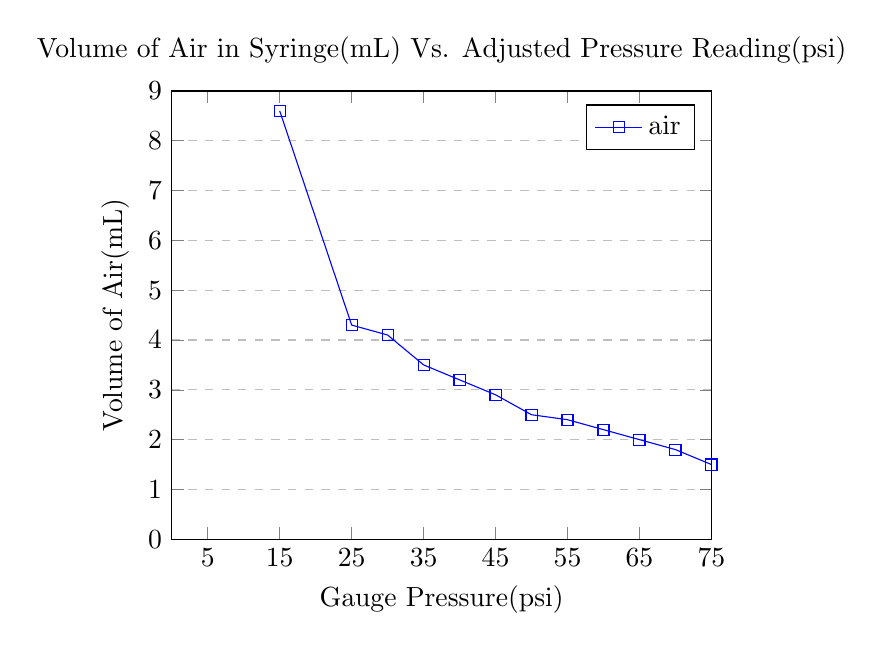
\begin{tikzpicture}
\begin{axis}[
    title={Volume of Air in Syringe(mL) Vs. Adjusted Pressure Reading(psi)},
    xlabel={Gauge Pressure(psi)},
    ylabel={Volume of Air(mL)},
    ymin=0, ymax=9,
    xmin=0, xmax=75,
    xtick={5,15,25,35,45,55,65,75},
    ytick={0, 1, 2, 3, 4, 5, 6, 7, 8, 9},
    legend pos=north east,
    ymajorgrids=true,
    grid style=dashed,
]

\addplot[
    color=blue,
    mark=square,
    ]
    coordinates {
    (75, 1.5)(70, 1.8)(65, 2.0)(60, 2.2)(55, 2.4)(50, 2.5)(45, 2.9)(40, 3.2)(35, 3.5)(30, 4.1)(25, 4.3)(15, 8.6)
    };
    \legend{air}
    
\end{axis}
\end{tikzpicture}

\end{minipage}
\centering
\textbf{Figure 1}: Inverse relationship between gauge pressure and volume
$\ $

\textbf{Figure 2}: Linear relationship between the inverse of volume and gauge pressure

This shows the inversely proportional affect of changing the pressure of a gas on its volume per Boyle's law. The high r\^2 value in the relationship between 1/Volume and Pressure demonstrates that this relationship is truly inverse.
\subsection{Activity 4}
In order to be used for the gas laws, it is best for the values to be in kelvin, with absolute units of temperature, so the units are converted like follows: $22^\circ C+273.15 = 295$


\centering
\begin{minipage}{0.4\textwidth}
\begin{table}[H]
    \begin{tabularx}{400pt}{p{1.7cm}|p{1cm}|p{1cm}|p{1cm}|} &Temp. ($^\circ C$) &Temp. (K)& Syringe Volume(mL) \\ \cline{1-4}
    Ambient&22&295&17\\
    Saltwater-Ice&0&273&12\\
    Ice Only&10&283&15\\
    Hot Water&76&349&20\\
    
    \end{tabularx}
\end{table}
\end{minipage}
\hfill
\begin{minipage}{0.5\textwidth}
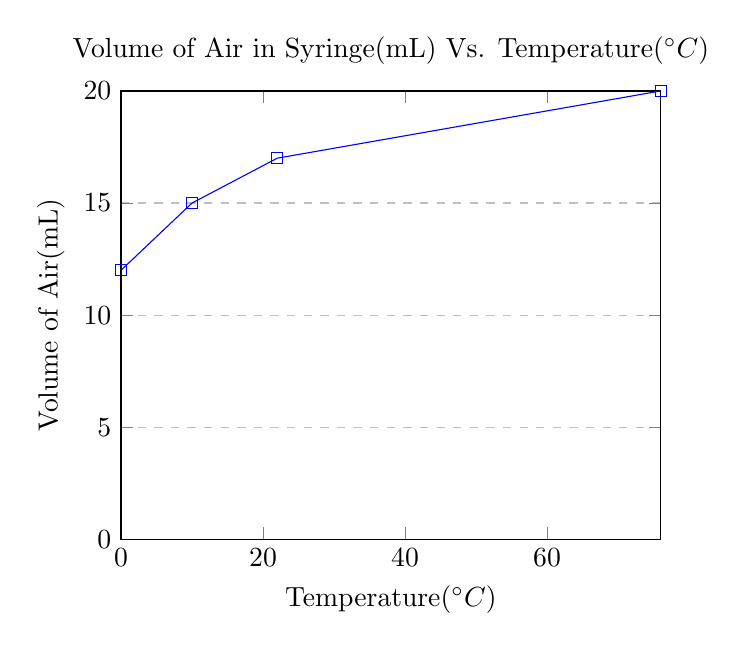
\begin{tikzpicture}
\begin{axis}[
    title={Volume of Air in Syringe(mL) Vs. Temperature($^\circ C$)},
    xlabel={Temperature($^\circ C$)},
    ylabel={Volume of Air(mL)},
    ymin=0, ymax=20,
    xmin=0, xmax=76,
    xtick={0,20,40,60,80},
    ytick={0,5,10,15,20},
    ymajorgrids=true,
    grid style=dashed,
]

\addplot[
    color=blue,
    mark=square,
    ]
    coordinates {
    (0,12)(10,15)(22,17)(76,20)
    };

\end{axis}
\end{tikzpicture}

\end{minipage}


$\ $

\textbf{Figure 3}: Linear relationship between temperature and volume

\textbf{Figure 4}: Linear relationship between temperature and volume

This shows the affect of changing the temperature of a gas on its volume per Charles' law.
\section{Discussion}
\subsection{Activity 1: Diffusion of Gases}
\begin{enumerate}
        \item The design of the divided petri plate ensures that the liquid ammonia cannot pass into the compartment with the Phenolphthalein indicator as it may not pass through the plastic barrier in liquid form.  However, as some particles with greater random velocity exit the ammonia compartment and enter the Phenolphthalein half of the petri dish, they make the Phenolphthalein turn violet.
        \item One example of this is the smell of liquids like isopropyl alcohol.  Isopropyl alcohol has a very low boiling point, so it is easy for liquid particles to be in gaseous form and a larger proportion of particles are in this gaseous and smell-able phase at one time.  Another example of this is the smell of the ocean, which has various smell-able particles which exit and travel with the wind as gases so we can smell what we associate with the ocean.
    \end{enumerate}
\subsection{Activity 2: Crush the Can}
    \begin{enumerate}
        \item As I explained above, the volume of air getting smaller inside the can made the can get smaller to accommodate this smaller volume. The actual force changing the volume is the atmospheric air pressure, and the "want" of air pressure inside the can and outside to be the same, or in equilibrium. Volume decreases to equalize this pressure, as $P\propto \frac{1}{V}$
        \item The air in the can was heated, so per Charles' law, the volume of the air got larger.  The can had an opening for it to escape, so when the air's volume got larger than the can, it took the path of least resistance and effused at a high rate. In a way, the boiling water drove the air out of the can as quickly-moving water molecules caused the heating of the air itself, however, the water itself didn't 'push' the air out as much as the air effused.
        \item There was less pressure after it was cooled because the temperature decreased and per Gay-Lussac's law($T\propto P$), pressure should decrease as well. The pressure decreases because the particles aren't moving as fast so they're colliding with the container's walls less frequently. 
    \end{enumerate}
\subsection{Activity 3: Boyle's Law}
    \begin{enumerate}
        \item The 10-mL syringe decreased in volume because the pressure on the molecules was increasing. On a molecular level, the same number of particles are colliding with the container more frequently at the same temperature(average speed per kinetic-molecular theory), so the only remaining factor to change is volume.  When volume gets smaller, the pressure must increase as there are fewer non-collision-with-container places for the particles to be, so the number of collisions increases.
        \item We observed the syringe first get smaller as we pumped up the bottle, increasing the air pressure, and then get larger as we let air out, decreasing the air pressure.  This simple observation alone indicates that air pressure is inversely proportional to volume, but the quantitative results really confirm it. Boyle's law states that $P \propto \frac{1}{V}$, so volume decreasing as pressure increased confirmed it.
        \item The general inverse shape of the Volume-Pressure graph suggested an inverse correlation, but the linear nature of the 1/Volume by Adjusted Pressure graph with a high coefficient of determination indicates that this correlation is present and very strong.  Boyle's law states that $P \propto \frac{1}{V}$, so we would expect an inverse relationship between the two, and that is certainly what we observe.
    \end{enumerate}
\subsection{Activity 4: Charles' Law}
\begin{enumerate}
        \item The mathematical relationship between temperature and volume of a gas is best described by Charles' law($T\propto V$), which says that pressure and volume are proportonal.  This means that as one increases the other increases and that as one decreases, the other decreases.  It also means that the amount of increase/decrease in one value per one unit increase in the other value is the same no matter what value.  
        \item This makes sense in terms of kinetic-molecular theory because as temperature increases, the average velocity of the particles increases, which means that they will hit the walls of the container more often just by virtue of being in different places more often.  Pressure is defined by the rate at which a particle hits the walls of its container, so pressure increases with temperature.
    \end{enumerate}
\end{document}
